\section{Product Brief}\label{product-brief}

\subsection{Introduction}\label{introduction}

The RV12 is a highly configurable single-issue, single-core RV32I, RV64I
compliant RISC CPU intended for the embedded market. The RV12 is a
member of the Roa Logic's 32/64bit CPU family based on the industry
standard RISC-V instruction set.

\begin{figure}[hbt]
  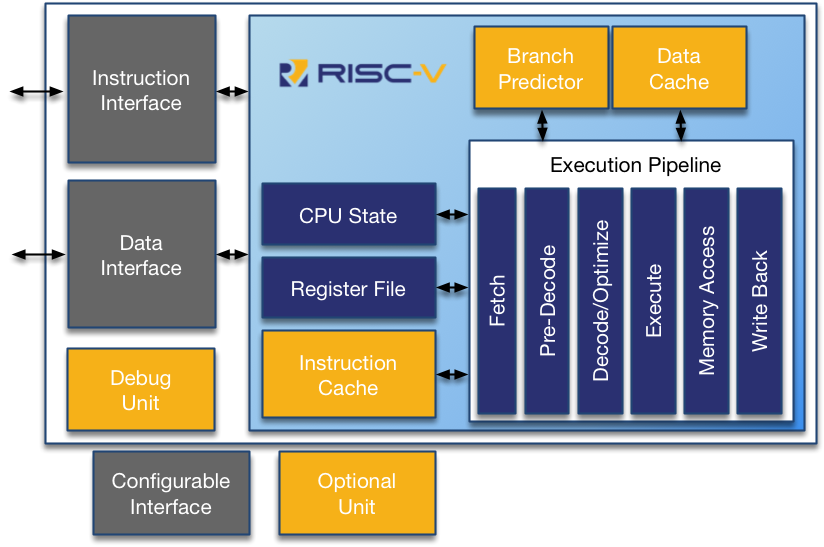
\includegraphics{RV12_Arch}
  \caption{RV12 Architecture}
\end{figure}

The RV12 implements a Harvard architecture for simultaneous instruction
and data memory accesses. It features an optimizing folded 4-stage
pipeline, which optimizes overlaps between the execution and memory
accesses, thereby reducing stalls and improving efficiency.

Optional features include Branch Prediction, Instruction Cache, Data
Cache, Debug Unit and optional Multiplier/Divider Units. Parameterized
and configurable features include the instruction and data interfaces,
the branch-prediction-unit configuration, and the cache size,
associativity, replacement algorithms and multiplier latency. Providing
the user with trade offs between performance, power, and area to
optimize the core for the application.

RV12 is compliant with the RISC-V User Level ISA v2.2 and Privileged
Architecture v1.9.1 specifications published by the RISC-V Foundation
(https://riscv.org).

\subsection{Features}\label{features}

\textbf{High Performance 32/64bit CPU}

\begin{itemize}
\item
  Royalty Free Industry standard instruction set (www.riscv.org)
\item
  Parameterized 32/64bit data
\item
  Fast, precise interrupts
\item
  Custom instructions enable integration of proprietary hardware
  accelerators
\item
  Single cycle execution
\item
  Optimizing folded 4-stage pipeline
\item
  Optional/Parameterized branch-prediction-unit
\item
  Optional/Parameterized caches
\end{itemize}

\textbf{Highly Parameterized}

\begin{itemize}
\item
  User selectable 32 or 64bit data
\item
  User selectable Branch Prediction Unit
\item
  User selectable instruction and/or data caches
\item
  User selectable cache size, structure, and architecture
\item
  Hardware Multiplier/Divider Support with user defined latency
\item
  Flexible bus architecture supporting AHB, Wishbone
\end{itemize}

\textbf{Size and power optimized design}

\begin{itemize}
\item
  Fully parameterized design provides power/performance tradeoffs
\item
  Gated clock design to reduce power
\item
  Small silicon footprint; 30kgates for full featured implementation
\end{itemize}

\textbf{Industry standard software support}

\begin{itemize}
\item
  Eclipse IDE for Windows/Linux
\item
  GNU Compiler Collection, debugger, linker, assembler
\item
  Architectural simulator
\end{itemize}
